\chapter{Kinematic Cuts}
\label{cha:KinematicCuts}

\section{SIDIS Cuts}
\label{sec:SIDISCuts}
After identifying particles, kinematic cuts must be implemented to insure the events are within the SIDIS region of phase space.
In order to remove exclusive events as well as events that are not in the deeply inelastic region, the conditions $W > 2.05\ \text{GeV}$ and $Q^2 > 1.0\ \text{GeV}^2$ are imposed.
Traditionally, the $z$ range for SIDIS is $0.4 < z < 0.7$, however, since the results of this analysis are binned in $z$, no cut is applied to $z$ and the entire $z$ range is analyzed.
Note that a missing mass cut has already been applied at the hadron identification stage, as described in chapter~\ref{cha:hadronID}.
%%%%%%%% maybe put a figure here

\section{$\phi_h$ Fiducial Cuts}
\label{sec:phihFiducialCuts}
Certain regions of $x$-$Q^2$-$z$-$P_{h\perp}^2$ space have limited $\phi_h$ coverage (due to acceptance).
The ``holes'' in the $\phi_h$ distribution occur around $\phi_h = 0$ a vast majority of the time.
As the edge of a hole is approached, the number of events begins to drop sharply.
This ``edge effect'' is difficult to describe realistically with simulations (simulations and acceptance studies are discussed in chapter~\ref{cha:MonteCarlo}), therefore a cut is applied to eliminate these regions.

For example, figure~\ref{fig:rec_pip_phih_x3_QQ0_z7_PT21} shows the $\pi^+$ $\phi_h$ distribution for $0.4 < x < 0.5$, $2.2 < Q^2 < 2.8 \text{GeV}^2$, $0.35 < z < 0.4$, and $0.05 < P_{h\perp}^2 < 0.1$.
It can be seen that just inside of $\pm 50^\circ$ the number of events begins to drop off to zero.
In this example, events with $-50^\circ < \phi_h < 50^\circ$ are cut to eliminate the edges.
Every $x$-$Q^2$-$z$-$P_{h\perp}^2$ bin has a different $\phi_h$ fiducial cut (if a cut is necessary) which was determined by eye, placing the cut at the location in $\phi_h$ where the distribution starts dropping off to zero.
%
\begin{figure}[htp]
\centering
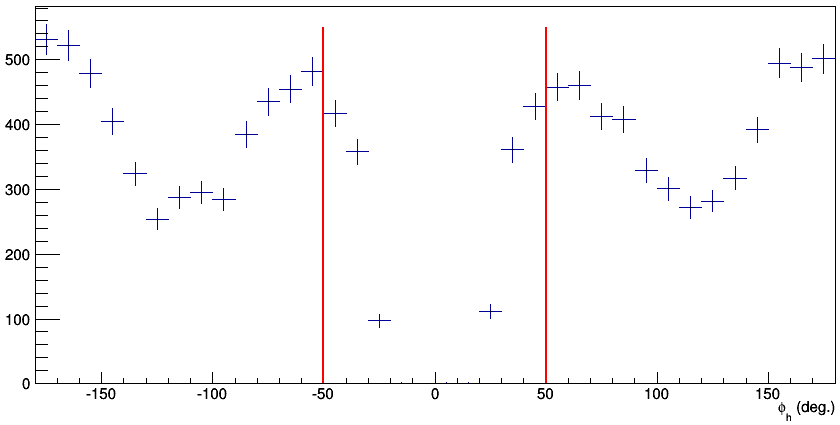
\includegraphics[width=4in]{figures/rec_pip_phih_x3_QQ0_z7_PT21.png}
\caption{The $\pi^+$ $\phi_h$ distribution for $0.4 < x < 0.5$, $2.2 < Q^2 < 2.8 \text{GeV}^2$, $0.35 < z < 0.4$, and $0.05 < P_{h\perp}^2 < 0.1$. The vertical red lines show the $\phi_h$ fiducial cut for this particular bin; events inside of the lines are cut to eliminate edge effects.}
\label{fig:rec_pip_phih_x3_QQ0_z7_PT21}
\end{figure}
%
